% !TeX spellcheck = en_US
\documentclass[12pt,fleqn]{article}


\usepackage[english]{babel}
\usepackage{amsmath}

\usepackage{texfiles/SpeedyGonzales}
\usepackage{texfiles/MediocreMike}
\usepackage{multicol}
\usepackage{subcaption}


\title{\vspace*{-3.75cm}Title}
\author{Søren Holm, Oskar Wiese, Anders Henriksen and Anne Pedersen \\
	\small {\texttt{\{s183911,s183917,s183904,s174300\}@student.dtu.dk}}}
\date{\today}


\pagestyle{fancy}
\fancyhf{}
\lhead{Title}
\rfoot{Page \thepage{} of \pageref{LastPage}}

\graphicspath{{imgs/}}

\begin{document}
	
	\maketitle
	 
	
	\begin{abstract} %TODO: Write section
		
	\end{abstract}
	
	\begin{multicols}{2}
		
		
		\section{Introduction} %TODO: Add something about GP
		The novel corona virus COVID-19 has affected the lives of billions of people all around the world. This project has collected a dataset of different measures for each country and then uses uncertainty sampling to classify countries by the number of COVID-19 related fatalities. Lastly we compare different ways of sampling to find the one that gets a satisfying accuracy the fastest. Our initial hypothesis is that margin sampling performs better than the other samplers due to the relatively small amount of classes. 
		
		\section{Data} 
		Our dataset was constructed from several different sources \cite{density, corona, alder, bnp, region, healthcare, turist}. For each country in the world with at least one COVID-19 related fatality, we collected eight features; the country's GDP per capita, population density per km$^2$, world region, median age of the population, index of quality of healthcare system, number of tourists per year in thousands, and the population count. These features were used to classify the countries by amount of deaths. 30 \% of the data was used for testing, while the remaining 70 \% was used for training. %TODO: Update data split

		\section{Methods}
		\subsection{Gaussian process} %TODO: Write section
		A Gaussian process was first used in order to estimate uncertainty...
		
		
		\subsection{Pool-based sampling}
		Pool-based sampling is a cycle of the learner getting a labeled dataset, training the model and then evaluating on an unlabeled test set. The labels subset of the unlabeled pool that the learner was most uncertain about are then queried and the samples are added to the training set. Then the cycle repeats until the model reaches a satisfying level of accuracy.  
		
		\subsection{Uncertainty sampling}
		There are different ways for a learner to query for labels from the unlabeled pool. This project implements uncertainty sampling, which uses a model to estimate the uncertainty of its predicted labels and then queries the data with the most uncertainty. Since this is a multi-class classification problem, there are different approaches to determining $x^*$; these include least confident, margin sampling and entropy. 
		
		\textbf{Least confident} identifies the datapoint with the lowest probability for its most likely label as
		
		$$x^*=\underset{x\in U}{\text{argmax}}(1-p_\theta(\hat{y}|x))$$ 
		
		where $x$ is each datapoint in the unlabeled pool $U$, and $\hat{y}=\underset{y\in Y}{\text{argmax}}(p_\theta(y|x))$ is the probability of the most likely label. 
		
		\textbf{Margin sampling} also takes into account the the second most likely label of $x$, $\hat{y}_2$ and then queries the datapoint with the smallest difference between $\hat{y}_1$ and $\hat{y}_2$:
		
		$$x^*=\underset{x\in U}{\text{argmin}}(p_\theta(\hat{y}_1|x)-p_\theta(\hat{y}_2|x))$$
		
		In theory, this would work well for a small number of labels. 
		
		\textbf{Entropy}, on the other hand, uses the full distribution of the labels and is therefore good for classification problems with a large number of labels:
		
		$$x^*=\underset{x\in U}{\text{argmax}}\left(-\sum_{y\in Y}p_\theta(y|x)\log p_\theta(y|x)\right)$$
		 
		The project aims to compare the performance of least confident, margin sampling and entropy on the proposed classification problem. 
		 
	\end{multicols}		

	\section{Results} %TODO: Write section
			\begin{figure}[H]
			\centering
			\begin{minipage}{.5\textwidth}
				\centering
				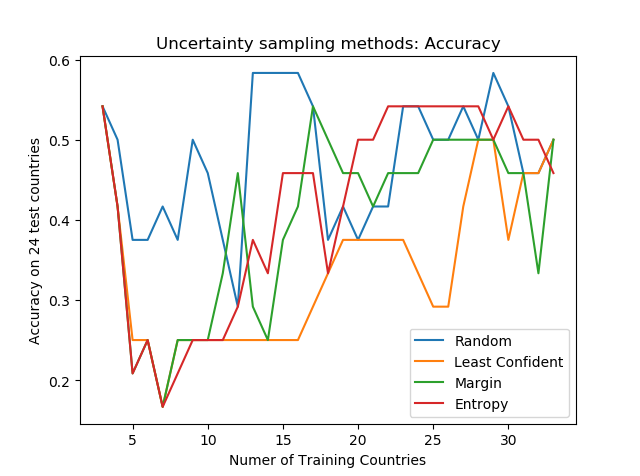
\includegraphics[width=\linewidth]{../src/saved_data/Accuracies}
				\caption{The accuracies of all four uncertainty sampling methods for every iteration.}
				\label{fig:accuracies}
			\end{minipage}%
			\begin{minipage}{.5\textwidth}
				\centering
				\includegraphics[width=\linewidth]{"../src/saved_data/Class balancing"}
				\caption{The proportion of the largest class in the pool at each iteration. Balance is at 0.33}
				\label{fig:class-balancing}
			\end{minipage}
			\end{figure}
			
		
	\begin{multicols}{2}

		\section{Discussion} %TODO: Write section
			
		\section{Learning outcome} %TODO: Write section
		Throughout the process of conducting the experiment and writing the report, a deeper understanding of the implementation and inner workings of active learning and uncertainty sampling and has been achieved. The unintuitive result of random sampling being close to on par with other methods has shown to not generally be the case but is rather caused by the class imbalance created when sampling from the pool. Realizing this allows for counteractive measures to be taken in the future to uphold this balance. Other minutia like increasing number of optimizer restarts and using an appropriate kernel have also proved to play an important role for sensible results.
			
	\end{multicols}

\newpage
\texttt{Code available at \url{github.com/sorenmulli/active_learning_cases}}
	\begin{thebibliography}{9}
	
	
		
		\bibitem{density} Wikipedia contributors: "List of countries and dependencies by population density", Date of last revision: 22 March 2020 15:25 UTC. Visited at,  \url{ https://en.wikipedia.org/w/index.php?title=List_of_countries_and_dependencies_by_population_density&oldid=946809073}
		
		\bibitem{corona} Balaaje from Kaggle: "Coronavirus (COVID-19) dataset" with data from \url{https://www.worldometers.info/coronavirus/}. Visited at, \url{https://www.kaggle.com/balaaje/coronavirus-covid19-dataset}
		
		\bibitem{alder} World Population Review: "Countries by Median Age 2018". Visited at, \url{https://worldpopulationreview.com/countries/median-age/}
		
		\bibitem{bnp} International Monetary Fund: "GDP per capita, current prices", ©IMF, 2019. Visited at, \url{https://www.imf.org/external/datamapper/NGDPDPC@WEO/OEMDC/ADVEC/WEOWORLD}
		
		\bibitem{region} J. SnowLabs, Datahub.io: "Country and Continent Codes List" . Can be found at, \url{https://datahub.io/JohnSnowLabs/country-and-continent-codes-list}
		
		\bibitem{healthcare} Numbeo.com: "Health Care Index by Country 2020". Visited at, \url{https://www.numbeo.com/health-care/rankings_by_country.jsp}
		
		\bibitem{turist} World Economic Forum: "Travel and Tourism Competitiveness Index", © 2020 World Economic Forum. Visited at, \url{http://reports.weforum.org/travel-and-tourism-competitiveness-report-2019/rankings/}
		
		
		
		
		
	\end{thebibliography}
	
	%\section{Appendix}
	
	
\end{document}

















